\documentclass[12pt]{exam}
\usepackage[margin=.6in,papersize={8.5in,17in}]{geometry}
\usepackage{enumitem}
\usepackage{tikz}
\usepackage{newtxtext,newtxmath}
\usepackage{bm}
\usepackage{siunitx}
\usepackage{circuitikz}

\setlength{\parindent}{0pt}
\setlength{\headheight}{14pt}

\usetikzlibrary{patterns}

\pagestyle{headandfoot}
\header{}{}{}
\footer{}{}{}

\newcommand{\pic}[2]{
  \begin{center}
    \includegraphics[width=#1\textwidth]{#2}
  \end{center}
}

\sisetup{
  inter-unit-product =\ensuremath{\cdot{}},
  per-mode=symbol
}
\tikzset{
  >=latex,
  voltage dir=RP
}


\renewcommand{\choiceshook}{
  \setlength{\leftmargin}{22pt}
  \setlength{\itemsep}{1.8pt}%.9\baselineskip}
  \setlength{\topsep}{0pt}
  \setlength\parsep{0pt}
}
\renewcommand{\choicelabel}{(\thechoice)}


\begin{document}

\begin{center}
  \textbf{AP \& IBHL PHYSICS PRACTICE TEST \#2\\
    PART 1: MULTIPLE-CHOICE QUESTIONS
  }
\end{center}

\textbf{Questions \ref{cylinder1}--\ref{cylinder2}:} A sealed cylinder with a
moveable piston contains $N$ molecules of an ideal gas. The gas is initially in
state $A$ shown on the above $PV$ diagram, where $P$ is pressure and $V$ is
volume. The gas is then taken through the two processes shown.
\begin{center}
  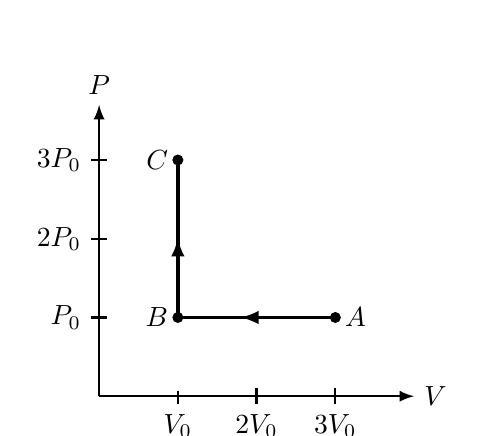
\begin{tikzpicture}
    \begin{scope}[thick]
      \draw[->](0,0)--(4,0) node[right]{$V$};
      \draw[->](0,0)--(0,3.7) node[above]{$P$};
      \draw(1,.07)--(1,-.1) node[below]{$V_0$};
      \foreach\x in {2,3} \draw(\x,.1)--(\x,-.1) node[below]{\x$V_0$};
      \draw(.1,1)--(-.1,1) node[left]{$P_0$};
      \foreach\y in {2,3} \draw(.1,\y)--(-.1,\y) node[left]{\y$P_0$};
    \end{scope}
    \fill (3,1) circle(.07) node[right]{$A$};
    \fill (1,1) circle(.07) node[left] {$B$};
    \fill (1,3) circle(.07) node[left] {$C$};
    \draw[very thick](3,1)--(1,1)--(1,3);
    \draw[very thick,->](3,1)--(1.8,1);
    \draw[very thick,->](1,1)--(1,2);
  \end{tikzpicture}
\end{center}

\begin{questions}
  \question Which of the following correctly ranks the average speed $\varv$ of
  the molecules in states $A$, $B$, and $C$?
  \label{cylinder1}
  \begin{choices}
    \choice $(\varv_B=\varv_C)>\varv_A$
    \choice $\varv_C>\varv_B>\varv_A$
    \choice $(\varv_A=\varv_C)>\varv_B$
    \choice $\varv_B>(\varv_C=\varv_A)$
  \end{choices}

  \question Which of the following correctly ranks the magnitude of the force
  $F$ the gas exerts on the piston in states $A$, $B$, and $C$?
  \label{cylinder2}
  \begin{choices}
    \choice $F_A>F_C>F_B$
    \choice $F_C>F_B>F_A$
    \choice $(F_B=F_C)>F_A$
    \choice $F_C>(F_A=F_B)$
  \end{choices}

  \question A sample of ideal gas in a tank of contant volume. The sample
  absorbs heat energy so that its temperature changes from \SI{300}{\kelvin} to
  \SI{600}{\kelvin}. If $\varv_1$ is the average speed of the gas molecules
  before the absorption of heat and $\varv_2$ is their average speed after the
  absorption of heat, what is the ratio $\varv_2/\varv_1$?
  \begin{choices}
    \choice $\dfrac12$
    \choice 1
    \choice $\sqrt2$
    \choice 2
    \choice 4
  \end{choices}
  
  \question A cylindrical resistor is connected to a battery with an emf of
  \SI{15.}{\volt}, resulting in a current of \SI{3.}{\ampere} in the circuit.
  The resistor is removed, and a new resistor of the same material with twice
  the radius and twice the length of the original resistor is connected to the
  battery. What is the new current in the circuit?
  \begin{choices}
    \choice \SI{1.5}{\ampere}
    \choice \SI{3.}{\ampere}
    \choice \SI{6.}{\ampere}
    \choice \SI{12.}{\ampere}
  \end{choices}

  \question Water of density \SI{1000}{\kilo\gram\per\metre\cubed} is pumped
  through a straight, horizontal hose and out a nozzle that has an opening with
  a cross-sectional area 10 times smaller than that of the hose. The water
  exits the nozzle at a speed of \SI{10.}{\metre\per\second}. The difference
  between the pressure of the fluid when it is in the hose near the pump and as
  it exits the nozzle is
  \begin{choices}
    \choice \SI{4.5e3}{\pascal}
    \choice \SI{4.95e4}{\pascal}
    \choice \SI{9.9e4}{\pascal}
    \choice \SI{4.95e6}{\pascal}
  \end{choices}

  \uplevel{
    \vspace{-.2in}
    \pic{.25}{rc1}
  }
  \question\vspace{-.2in}In the circuit shown above, bulbs $X$, $Y$, and $Z$
  are identical and capacitor $C$ is initially uncharged. The switch is closed
  at time $t=0$. Which of the following describes the brightness of bulbs $Y$
  and $Z$ after the switch is closed?
  \begin{choices}
    \choice Both bulbs light and remain lit.
    \choice Bulbs $Y$ and $Z$ are both initially lit, and bulb $Y$ eventually
    goes out.
    \choice Bulbs $Y$ and $Z$ are both initially lit, and bulb $Z$ eventually
    goes out.
    \choice Bulb $Y$ is always lit and bulb $Z$ is always out.
  \end{choices}
  \vspace{.6in}

  \uplevel{
    \textbf{Questions \ref{circuit1}--\ref{circuit2}} refer to the following
    diagram that shows part of a closed electrical circuit.
    \begin{center}
      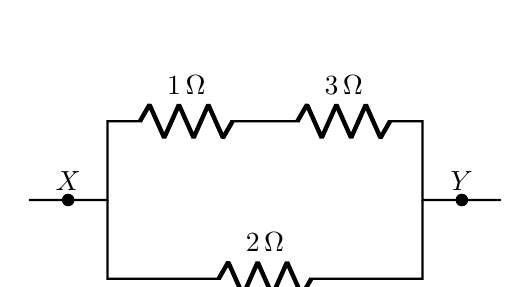
\begin{tikzpicture}
        \draw[thick](0,0)--(1,0)--(1,1)to[R,l=\mbox{\SI1{\ohm}}](3,1)
        to[R,l=\mbox{\SI3{\ohm}}](5,1)--(5,0)--(6,0);
        \draw[thick](1,0)--(1,-1) to[R,l=\mbox{\SI2{\ohm}}](5,-1)--(5,0);
        \fill( .5,0) circle(.08) node[above]{$X$};
        \fill(5.5,0) circle(.08) node[above]{$Y$};
      \end{tikzpicture}
    \end{center}
  }
  \question The electrical resistance of the part of the circuit shown between
  point $X$ and point $Y$ is:
  \label{circuit1}
  \begin{choices}
    \choice $1\dfrac13\si{\ohm}$
    \choice \SI2{\ohm}
    \choice $2\dfrac34\si{\ohm}$
    \choice \SI4{\ohm}
    \choice \SI6{\ohm}
  \end{choices}

  \question When there is a steady current in the circuit, the mount of
  charg passing a point per unit time is
  \label{circuit2}
  \begin{choices}
    \choice the same everywhere in the circuit
    \choice greater at $X$ than at point $Y$
    \choice greater in the \SI1{\ohm} than the \SI2{\ohm} resistor
    \choice greater in the \SI1{\ohm} than the \SI3{\ohm} resistor
    \choice greater in the \SI2{\ohm} than the \SI3{\ohm} resistor
  \end{choices}
  
  \question A student in a classroom sees a tree outside that is far from the
  classroom window and uses a concave mirror to form an image of the tree on a
  screen. Which of the following best describes the image?
  \begin{choices}
    \choice Real and near the center of curvature of the mirror
    \choice Real and near the focal point of the mirror
    \choice Virtual and near the center of curvature of the mirror
    \choice Virtual and near the focal point of the mirror
  \end{choices}

  \question A concave mirror with a radius of curvature of \SI{1.}{\metre} is
  used to collect light from a distant star. The distance between the mirror and
  the image of the star is most nearly
  \begin{choices}
    \choice 0.25 m
    \choice 0.50 m
    \choice 0.75 m
    \choice 1.0 m
    \choice 2.0 m
  \end{choices}

  \uplevel{
    \centering
    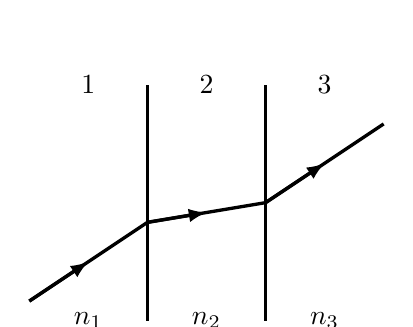
\begin{tikzpicture}[xscale=1.5]
      \draw[thick](1,0)--(1,3);
      \draw[thick](2,0)--(2,3);
      \draw[very thick](0,.25)--(1,1.25)--(2,1.5)--(3,2.5);
      \draw[very thick,->](0,.25)--(.5,.75);
      \draw[very thick,->](1,1.25)--(1.5,1.375);
      \draw[very thick,->](2,1.5)--(2.5,2);
      \foreach \x in {1,...,3}{
        \node at (\x-.5,0) {$n_\x$};
        \node at (\x-.5,3) {\x};
      }
    \end{tikzpicture}
  }
  \question A light ray passes through substances 1, 2, and 3, as shown above.
  The indices of refraction for these three substances are  $n_1$, $n_2$, and
  $n_3$, respectively. Ray segment in 1 and 3 are parallel. From the direction
  of the ray, one can conclude that
  \begin{choices}
    \choice $n_3$ must be the same as $n_1$
    \choice $n_2$ must be the same as $n_1$
    \choice $n_2$ must be the same as $n_3$
    \choice $n_1$ must be equal to 1.00
    \choice all three indices must be the same
  \end{choices}
  
  \uplevel{
    \vspace{-.3in}
    \pic{.5}{prism-aquarium}
  }
  \question\vspace{-.2in}A beam of white light is incident on a triangular
  glass prism with
  an index of refraction of about 1.5 for visible light, producing a spectrum.
  Initially, the prism is in a glass aquarium filled with air, as shown above.
  If the squarium is filled with water with an index of refraction of 1.3, which
  of the following is true?
  \begin{choices}
    \choice No spectrum is produced.
    \choice A spectrum is produced, but the deviation of the beam is opposite
    to that in the air.
    \choice The position of red and violet are reversed in the spectrum.
    \choice The spectrum produced has greater separation between red and violet
    than that produced in air.
    \choice The spectrum produced has less separation between red and violet
    than that produced in air.
  \end{choices}
  \newpage

  \question When light passes from air into water, the frequency of the light
  remains the same. What happens to the speed and wavelength of the light as
  it crosses the boundary in going from air into water?

  \begin{tabular}{cll}
    & Speed & Wavelength \\\hline
    (A) & Increases        & Remains the same \\
    (B) & Remains the same & Decreases        \\
    (C) & Remains the same & Remains the same \\
    (D) & Decreases        & Increases \\
    (E) & Decreases        & Decreases
  \end{tabular}
  
  \uplevel{
    \centering
    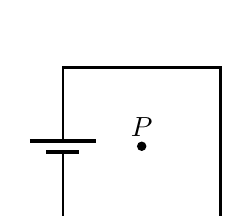
\begin{tikzpicture}
      \draw[thick](0,0) to[battery1](0,2)--(2,2)--(2,0)--(0,0);
      \fill(1,1) circle(.06) node[above]{$P$};
    \end{tikzpicture}
  }
  \question A circuit consists of a battery and some wire with significant
  resistance. The wire is bent so that the circuit is in the shape of a square,
  and the circuit is aligned in the plane of the page, as shown above. Which of
  the following best describes the direction of the magnetic field near point
  $P$?
  \begin{choices}
    \choice Clockwise around point $P$
    \choice Out of the page
    \choice Into the page
    \choice The field has no direction because the magnitude of the field is
    zero.
  \end{choices}
  
  \uplevel{
    \centering
    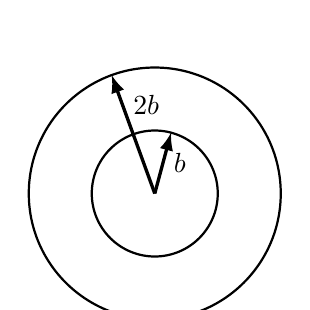
\begin{tikzpicture}[scale=.8]
      \draw[thick](0,0) circle(1);
      \draw[thick](0,0) circle(2);
      \draw[very thick,->,rotate=-15](0,0)--(0,1) node[midway,right] {$b$};
      \draw[very thick,->,rotate=20 ](0,0)--(0,2) node[pos=.75,right]{$2b$};
    \end{tikzpicture}
  }
  \question Two concentric loops of radii $b$ and $2b$, made of the same type of
  wire, lie in the plane of the page, as shown above. The total resistance of
  the wire loop of radius $b$ is $R$. What is the resistance of the wire loop
  of wire $2b$?
  \begin{choices}
    \choice $R/4$
    \choice $R/2$
    \choice $R$
    \choice $2R$
    \choice $4R$
  \end{choices}
  
  \uplevel{
    \vspace{-.3in}
    \pic{.3}{photoelectric1}
  }
  \question\vspace{-.2in}A photon with energy \SI{4}{\electronvolt} is incident
  on metal $X$, which has a work function of \SI{3}{\electronvolt}. Metal $X$ is
  electrically connected to metal $Y$ through a \SI{2}{\volt} voltage supply
  with the polarity shown in the figure above. What is the maximum kinetic
  energy an emitted electron could have when it reaches metal $Y$?
  \begin{choices}
    \choice \SI{1}{\electronvolt}
    \choice \SI{2}{\electronvolt}
    \choice \SI{3}{\electronvolt}
    \choice \SI{5}{\electronvolt}
  \end{choices}

  \question In an experiment, light of a particular wavelength is incident on
  a metal surface, and electrons are emitted from the surface as a result. To
  produce more electrons per unit time but with less kinetic energy per
  electron, the experimenter should do which of the following?
  \begin{choices}
    \choice Increase the intensity and decrease the wavelength of the light.
    \choice Increase the intensity and the wavelength of the light.
    \choice Decrease the intensity and the wavelength of the light.
    \choice Decrease the intensity and increase the wavelength of the light.
    \choice None of the above would produce the desired result.
  \end{choices}
  
  \uplevel{
    \centering
    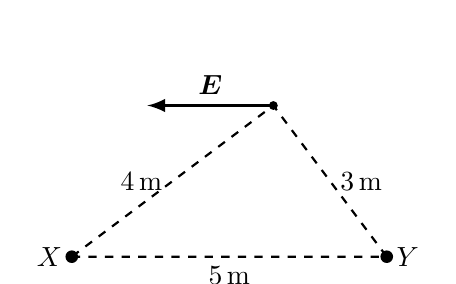
\begin{tikzpicture}[scale=.8]
      \coordinate(x) at (0,0);
      \coordinate(y) at (5,0);
      \coordinate(z) at ({4*cos(atan(3/4))},{4*sin(atan(3/4))});
      \draw[thick,dashed](x)--(y) node[midway,below]{\SI5\metre}
      --(z) node[midway,right]{\SI3\metre}--(x) node[midway,left]{\SI4\metre};
      \fill(x) circle(.1) node[left]{$X$};
      \fill(y) circle(.1) node[right]{$Y$};
      \fill(z) circle(.07);
      \draw[very thick,->](z)--+(-2,0) node[midway,above]{$\bm{E}$};
    \end{tikzpicture}
  }
  \question\vspace{-.1in}Two charged spheres, $X$ and $Y$, are held fixed at
  two vertices of
  a triangle, as shown above. The direction of the electric field $\bm{E}$ at
  the third vertex due to the two spheres is also shown. Which of the following
  correctly indicates the sign of the charges on the spheres?

  \begin{tabular}{ccc}
    & \textbf{Sphere $X$} & \textbf{Sphere $Y$} \\ \hline
    (A) & Positive & Positive \\
    (B) & Positive & Negative \\
    (C) & Negative & Positive \\
    (D) & Negative & Negative
  \end{tabular}

  \uplevel{
    \begin{minipage}{.49\linewidth}
      \pic{.7}{tapes}
    \end{minipage}
    \begin{minipage}{.49\linewidth}
      \centering
      \begin{tabular}{l|c|c}
        & \textbf{Tape 1} & \textbf{Tape 2}\\ \hline\hline
        Positively charged object & Attracted & Repelled \\
        Negatively charged object & Repelled  & Attracted \\
        Uncharged object          & Attracted & Attracted \\ \hline
      \end{tabular}
    \end{minipage}
  }
  
  \question\vspace{.2in}Two pieces of transparent adhesive tape, labeled 1 and 2, are stuck
  together. The pieces of tape are then quickly pulled apart and stuck to an
  insulating rod, as shown above. Three objects are brought near each piece of
  tape, one at a time. One of the objects is positively charged, one is
  negatively charged, and one is uncharged. The reaction of each piece of tape
  is recorded in the table above. Based on the results, what can be concluded
  about the signs of the charges on the tapes, and why?
  \begin{choices}
    \choice Tape 1 is positively charged, because it is attracted to the
    positively charged object. Tape 2 is negatively charged because it is
    repelled by the positively charged object.
    \choice Tape 1 is negatively charged, because it is repelled by the
    negatively charged object. Tape 2 is positively charged, because it is
    repelled by the positively charged object.
    \choice Tape 1 and tape 2 are both positively charged because they are both
    attracted to the uncharged object.
    \choice Tape 1 and tape 2 are both negatively charged because they are both
    attracted to the uncharged object.
  \end{choices}
  \vspace{.7in}

  \uplevel{
    \centering
    \begin{tikzpicture}[scale=1.2]
      \draw[very thick](2,.7) circle(.1);
      \draw[very thick,->](2.2,.7)--+(1,0);
      \draw[very thick](0,0)--(4,0);
      \draw[very thick,->](2,0)--(2.4,0);
    \end{tikzpicture}
  }
  \question At the instant shown above, a particle with a positive charge
  travels to the right near a wire carrying a current to the right. What is the
  direction of the force exerted by the charge on the wire?
  \begin{choices}
    \choice Toward the bottom of the page
    \choice Toward the top of the page
    \choice Out of the page
    \choice Into the page
  \end{choices}


  \uplevel{
    \centering
    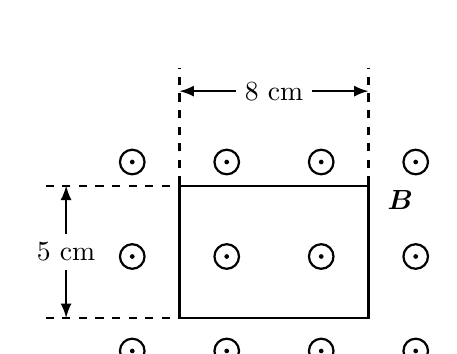
\begin{tikzpicture}[scale=1.2]
      \foreach \x in {0,...,3} {
        \foreach \y in {0,...,2} {
          \draw[thick] (\x,\y) circle(.13);
          \fill (\x,\y) circle(.025);
        }
      }
      \draw[thick](.5,.35) rectangle (2.5,1.75);
      \draw[thick,dashed](.4,0.35)--(-1,0.35);
      \draw[thick,dashed](.4,1.75)--(-1,1.75);
      \draw[thick,<->](-.7,1.75)--(-.7,0.35) node[midway,fill=white]{5 cm};
      \draw[thick,dashed](0.5,1.76)--(0.5,3);
      \draw[thick,dashed](2.5,1.76)--(2.5,3);
      \draw[thick,<->](.5,2.75)--(2.5,2.75) node[midway,fill=white]{8 cm};
      \node[right] at (2.6,1.6){$\bm B$};
    \end{tikzpicture}
  }
  \question A rectangular wire loop is at rest in a uniform magnetic field
  $\bm{B}$ of magnitude \SI{2}{\tesla} that is directed out of the page. The
  loop measures \SI{5}{\centi\metre} by \SI{8}{\centi\metre}, and the plane of
  the loop is perpendicular to the field, as shown above. The total magnetic
  flux through the loop is
  \begin{choices}
    \choice zero
    \choice \SI{2e-3}{\tesla.\metre\squared}
    \choice \SI{8e-3}{\tesla.\metre\squared}
    \choice \SI{2e-1}{\tesla.\metre\squared}
    \choice \SI{8e-1}{\tesla.\metre\squared}
  \end{choices}
  
  \question A beam of electrons is incident on a crystal, creating a
  diffraction pattern. How should the speed of the electrons be changed to
  increase the separation of the spacing of the maxima in the pattern, and why
  would the pattern change?
  \begin{choices}
    \choice The speed should be increased, because that would increase the de
    Broglie wavelength of the electrons.
    \choice The speed should be increased, because that would decrease the de
    Broglie wavelength of the electrons.
    \choice The speed should be decreased, because that would increase the de
    Broglie wavelength of the electrons.
    \choice The speed should be decreased, because that would decrease the de
    Broglie wavelength of the electrons.
  \end{choices}
  \vspace{.7in}
  
  \question A canister and the hydrogen gas it contains are at
  \SI{100}{\celsius}. The canister is placed in a vacuum, and the temperature
  of the canister and gas begins to decrease. Which of the following statements
  of reasoning best explains how the canistergas system loses energy?
  \begin{choices}
    \choice High-energy hydrogen molecules collide with lower-energy molecules
    and the walls inside the canister, losing energy during the collisions.
    \choice The molecules collide with the walls of the canister, causing the
    canister molecules to vibrate and carry energy from the canister to the
    canister's surroundings.
    \choice Energy is released from the canister as infrared radiation that can
    travel through the vacuum, causing a decrease in the average energy of the
    canister and the molecules.
    \choice Energy is released from the canister and travels through the vacuum
    by convection, causing a decrease in the average energy of the canister and
    the molecules.
  \end{choices}
  \vspace{.7in}
  
  \uplevel{
    \pic{.34}{energy-levels}
  }
  \question The figure above shows the energy levels for a hypothetical atom.
  For which transitions will the emitted photon have an energy of
  \SI{4}{\electronvolt}? Select two answers.
  \begin{choices}
    \choice $n=4$ to $n=3$
    \choice $n=4$ to $n=2$
    \choice $n=3$ to $n=1$
    \choice $n=2$ to $n=1$
  \end{choices}

  \question A student is asked to use the steps listed below to induce a
  positive charge on an aluminum soda can. In what order could the steps be
  done to accomplish the task? Select two answers.
  
  Step W: Bring a negatively charged rod near, but not touching, the can.

  Step X: Ground the can.

  Step Y: Remove the ground from the can.

  Step Z: Move the charged rod away from the can.
  \begin{choices}
    \choice W, X, Y, Z
    \choice W, X, Z, Y
    \choice X, W, Y, Z
    \choice X, W, Z, Y
  \end{choices}

  \uplevel{
    \centering
    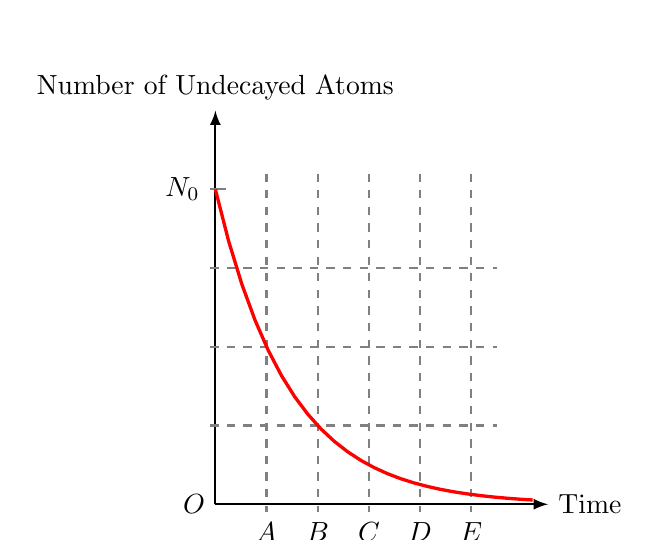
\begin{tikzpicture}[xscale=.65]
      \draw[thick,->](0,0)--(6.5,0) node[right]{Time} node[pos=0,left]{$O$};
      \draw[thick,->](0,0)--(0,5) node[above]{Number of Undecayed Atoms};
      \foreach \y in {1,...,3} \draw[thick,dashed,gray](-.1,\y)--(5.5,\y);
      \draw[thick,gray](.2,4)--(-.1,4) node[left,black]{$N_0$};
      \draw[thick,dashed,gray](1,4.2)--(1,-.1) node[below,black]{$A$};
      \draw[thick,dashed,gray](2,4.2)--(2,-.1) node[below,black]{$B$};
      \draw[thick,dashed,gray](3,4.2)--(3,-.1) node[below,black]{$C$};
      \draw[thick,dashed,gray](4,4.2)--(4,-.1) node[below,black]{$D$};
      \draw[thick,dashed,gray](5,4.2)--(5,-.1) node[below,black]{$E$};
      \draw[domain=0:6.2,very thick,red] plot(\x,{2^(-\x)*4});
    \end{tikzpicture}
  }
  
  \question The graph above shows the decay of a sample of carbon-14 that
  initially contained $N_0$ atoms.  Which of the lettered points on the time
  axis chould represent the half-life of carbon-14?
  \begin{choices}
    \choice $A$
    \choice $B$
    \choice $C$
    \choice $D$
    \choice $E$
  \end{choices}

  \question At noon a radioactive sample decays at a rate of \num{4000} counts
  per minute. At 12:30 pm the decay rate has decreased to \num{2000} counts per
  minute. The predicted decay rate at 1:30 pm is:
  \begin{choices}
    \choice 0 counts
    \choice 500 counts
    \choice 666 counts
    \choice \num{1000} counts
    \choice \num{1333} counts
  \end{choices}

  \question An ice cube of mass $m$ and specific heat $c_i$ is initially at
  temperature $T_1$, where $T_1<\SI{273}{\kelvin}$. If $L$ is the latent heat
  of fusion of water, and the specific heat of water is $c_w$, how much energy
  is required to convert the ice cube to water at temperature $T_2$ where,
  $\SI{273}{\kelvin}<T_2<\SI{373}{\kelvin}$?
  \begin{choices}
    \choice $m[c_i(273-T_1)+L+c_w(373-T_2)]$
    \choice $m[c_i(273-T_1)+L+c_w(T_2-273)]$
    \choice $c_i(273-T_1)+c_w(T_2-273)$
    \choice $mL+c_w(T_2-T_1)$
    \choice $mL+\left(\dfrac{c_w-c_i}{2}\right)(T_2-T_1)$
  \end{choices}
\end{questions}
\end{document}
